% This work is licensed under the Creative Commons
% Attribution-NonCommercial-ShareAlike 4.0 International License. To view a copy
% of this license, visit http://creativecommons.org/licenses/by-nc-sa/4.0/ or
% send a letter to Creative Commons, PO Box 1866, Mountain View, CA 94042, USA.



\tikzset{every picture/.style={line width=0.75pt}} %set default line width to 0.75pt        

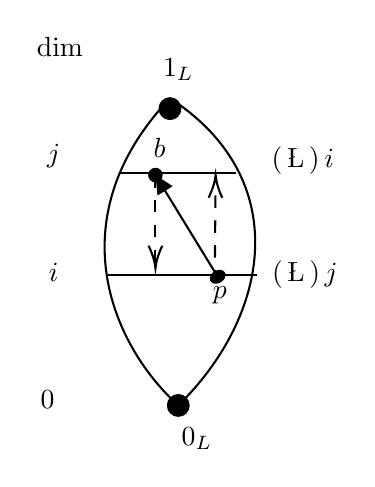
\begin{tikzpicture}[x=0.75pt,y=0.75pt,yscale=-1,xscale=1]
%uncomment if require: \path (0,300); %set diagram left start at 0, and has height of 300

%Curve Lines [id:da9559714668165431] 
\draw    (258,209.93) .. controls (225,179.93) and (200,118.93) .. (254,61.93) ;


%Curve Lines [id:da870462767582893] 
\draw    (258,209.93) .. controls (302,166.93) and (314,100.93) .. (254,61.93) ;


%Shape: Circle [id:dp6905850303089136] 
\draw  [fill={rgb, 255:red, 0; green, 0; blue, 0 }  ,fill opacity=1 ] (249,66.93) .. controls (249,64.17) and (251.24,61.93) .. (254,61.93) .. controls (256.76,61.93) and (259,64.17) .. (259,66.93) .. controls (259,69.69) and (256.76,71.93) .. (254,71.93) .. controls (251.24,71.93) and (249,69.69) .. (249,66.93) -- cycle ;
%Shape: Circle [id:dp3933822162001085] 
\draw  [fill={rgb, 255:red, 0; green, 0; blue, 0 }  ,fill opacity=1 ] (253,209.93) .. controls (253,207.17) and (255.24,204.93) .. (258,204.93) .. controls (260.76,204.93) and (263,207.17) .. (263,209.93) .. controls (263,212.69) and (260.76,214.93) .. (258,214.93) .. controls (255.24,214.93) and (253,212.69) .. (253,209.93) -- cycle ;
%Straight Lines [id:da2624167968218917] 
\draw    (230,97.93) -- (286,97.93) ;


%Straight Lines [id:da8790065247209863] 
\draw    (224,146.93) -- (296,146.93) ;


%Straight Lines [id:da09868631062113131] 
\draw    (248.04,100.64) -- (277,147.93) ;

\draw [shift={(247,98.93)}, rotate = 58.52] [fill={rgb, 255:red, 0; green, 0; blue, 0 }  ][line width=0.75]  [draw opacity=0] (8.93,-4.29) -- (0,0) -- (8.93,4.29) -- cycle    ;
%Shape: Circle [id:dp07389781898233405] 
\draw  [fill={rgb, 255:red, 0; green, 0; blue, 0 }  ,fill opacity=1 ] (244,98.93) .. controls (244,97.28) and (245.34,95.93) .. (247,95.93) .. controls (248.66,95.93) and (250,97.28) .. (250,98.93) .. controls (250,100.59) and (248.66,101.93) .. (247,101.93) .. controls (245.34,101.93) and (244,100.59) .. (244,98.93) -- cycle ;
%Shape: Circle [id:dp15699358050616063] 
\draw  [fill={rgb, 255:red, 0; green, 0; blue, 0 }  ,fill opacity=1 ] (274.03,147.49) .. controls (274.83,145.93) and (276.8,144.87) .. (278.43,145.11) .. controls (280.07,145.36) and (280.76,146.82) .. (279.97,148.38) .. controls (279.17,149.93) and (277.2,151) .. (275.57,150.75) .. controls (273.93,150.51) and (273.24,149.04) .. (274.03,147.49) -- cycle ;
%Straight Lines [id:da5019157895054271] 
\draw  [dash pattern={on 4.5pt off 4.5pt}]  (247,98.93) -- (247,141.93) ;
\draw [shift={(247,143.93)}, rotate = 270] [color={rgb, 255:red, 0; green, 0; blue, 0 }  ][line width=0.75]    (10.93,-3.29) .. controls (6.95,-1.4) and (3.31,-0.3) .. (0,0) .. controls (3.31,0.3) and (6.95,1.4) .. (10.93,3.29)   ;

%Straight Lines [id:da5990497530420301] 
\draw  [dash pattern={on 4.5pt off 4.5pt}]  (275.57,150.75) -- (275.98,100.93) ;
\draw [shift={(276,98.93)}, rotate = 450.48] [color={rgb, 255:red, 0; green, 0; blue, 0 }  ][line width=0.75]    (10.93,-3.29) .. controls (6.95,-1.4) and (3.31,-0.3) .. (0,0) .. controls (3.31,0.3) and (6.95,1.4) .. (10.93,3.29)   ;


% Text Node
\draw (201,37) node   {$\dim$};
% Text Node
\draw (258,48) node   {$1_{\mathbb{L}}$};
% Text Node
\draw (198,90) node   {$j$};
% Text Node
\draw (198,146) node   {$i$};
% Text Node
\draw (195,207) node   {$0$};
% Text Node
\draw (319,147) node   {$\begin{pmatrix}
	\L\\j
\end{pmatrix}$};
% Text Node
\draw (318,92) node   {$\begin{pmatrix}
	\L\\i
\end{pmatrix}$};
% Text Node
\draw (267,226) node   {$0_{\mathbb{L}}$};
% Text Node
\draw (249,86) node   {$b$};
% Text Node
\draw (278,157) node   {$p$};


\end{tikzpicture}
